%This work is licensed under the Creative Commons Attribution-NonCommercial-NoDerivs 3.0 United States License. To view a copy of this license, visit http://creativecommons.org/licenses/by-nc-nd/3.0/us/ or send a letter to Creative Commons, 444 Castro Street, Suite 900, Mountain View, California, 94041, USA.

\section{Magnetic Lenses} \label{sec:mag_lens}

%\subsection{Motivation}
% montgomery_some_1961
% el-kareh_electron_1970

In many ways, an electron beam can be thought of in terms of an optical equivalent system. 
Of course there are notable exceptions; photons don't repel each other; photon energies are hard to change.
Electron optical systems do have an analogous system to the lens, in this case using magnetic fields rather than glass. 
The magnetic lens is a common element in electron microscopes and other electron-optical systems.
%TODO refs needed

Magnetic lenses present some challenges for Ultrafast Electron Microscopy.
First, the beams are likely to be much larger and thus a UEM will need large-aperture lenses.
Second, and more importantly, near a lens crossover (i.e. focus), the charge density can increase rapidly.
This charge density can lead to an unacceptable amount of space-charge interaction.
These effects have been explored in Sections \ref{sec:free_spacecharge} and \ref{sec:mag_lens_charge}.
The lenses I present in this section were designed, in part, using information computed by the extended AG model (Section \ref{sec:mag_lens_model}).

\subsection{Design}

Discussion of the mathematics of magnetic lenses can be found in Section \ref{sec:mag_lens}.
While in principle one could design a magnetic lens using \ref{eq:lens_eq_of_motion} and \ref{eq:field_of_loop}, the process wouldn't be very practical or instructive.
Further --- as suggested by the use of the auxiliary field $H$ field in \ref{eq:field_of_loop} --- better performance of the lens can be achieved by concentrating the field using materials with high magnetic permeablility.
These materials, called ``magnetic shielding'' since it captures the magnetic field lines, can direct the field lines to a small gap, known as the ``pole-piece gap''.
The field lines exit the shielding in the gap and it is this field that acts as the lens.
This gap can be much smaller than the total width of the coil turns, and yet contain in a field commensurate with the full coil.

\begin{figure}
  \centering
  %This work is licensed under the Creative Commons Attribution-NonCommercial-NoDerivs 3.0 United States License. To view a copy of this license, visit http://creativecommons.org/licenses/by-nc-nd/3.0/us/ or send a letter to Creative Commons, 444 Castro Street, Suite 900, Mountain View, California, 94041, USA.

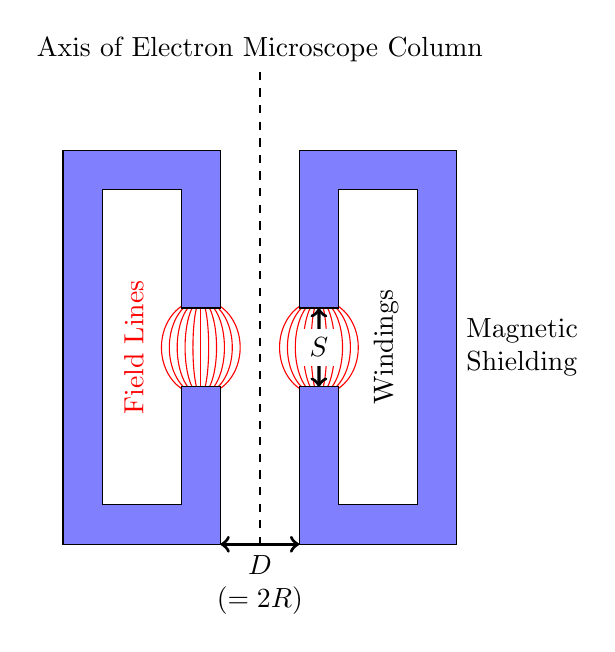
\begin{tikzpicture}
  \foreach \n in {0,0.1,...,0.6}{
    \draw [red] (0.75,-0.5) ellipse [x radius=\n,y radius=0.6];
  }
  \foreach \n in {0,0.1,...,0.6}{
    \draw [red] (-0.75,-0.5) ellipse [x radius=\n,y radius=0.6];
  }
  \draw [fill=blue!50] 
    (-0.5,0)
    -- ++(0,2)
    -- ++(-2,0)
    -- ++(0,-5)
    -- ++(2,0)
    -- ++(0,2)
      coordinate [pos=0] (D left)
    -- ++(-0.5,0)
    -- ++(0,-1.5)
    -- ++(-1,0)
    -- ++(0,4)
    -- ++(1,0)
    -- ++(0,-1.5)
    -- ++(0.5,0)
    -- cycle
  ;
  \draw [fill=blue!50] 
    (0.5,0)
    -- ++(0,2)
    -- ++(2,0)
    -- ++(0,-5)
      node [pos=0.5,right,align=left] {Magnetic\\Shielding}
    -- ++(-2,0)
    -- ++(0,2)
      coordinate [pos=0] (D right)
    -- ++(0.5,0)
      coordinate [pos=0.5] (S top)
    -- ++(0,-1.5)
    -- ++(1,0)
    -- ++(0,4)
    -- ++(-1,0)
    -- ++(0,-1.5)
    -- ++(-0.5,0)
      coordinate [pos=0.5] (S bottom)
    -- cycle
  ;
  \draw [thick, dashed]
    (0,3)
    -- (0,-3)
      node [pos=0,above] {Axis of Electron Microscope Column}
  ;
  \draw [very thick,<->] 
    (S top) 
    -- (S bottom)
      node [pos=0.5,fill=white] {$S$}
  ;
  \draw [very thick,<->] 
    (D left) 
    -- (D right)
      node [below,pos=0.5,align=center] {$D$\\$(=2R)$}
  ;
  \node [rotate=90] at (1.6,-0.5) {Windings};
  \node [red,rotate=90] at (-1.6,-0.5) {Field Lines};
\end{tikzpicture}

  \caption[Side-view schematic of a shielded magnetic lens with a pole-piece]{
    Side-view schematic of a shielded magnetic lens with a pole-piece.
    The windings (current loops) are contained within the shielding.
    The magnetic field created by these windings is contained inside the shielding except in the gap.
  }
\end{figure}

El-Kareh and El-Kareh \cite{el-kareh_electron_1970} provide an analysis of symmetric lenses with magnetic shielding and a pole-piece in chapter 8, with the most useful information being in section 8.7.
They define
\begin{subequations}
\begin{gather}
  k^2 \equiv \frac{e}{8 m V_r} B_0^2 R^2 \\
  \beta \equiv k^2 V_r / (NI)^2 \label{eq:elkareh_k2}
\end{gather}
\end{subequations}
where $N$ is the number of loops, $I$ is the current in a single loop, $B_0$ is the maximum axial magnetic field strength, $R$ is the bore radius and $V_r$ is the relativity corrected acceleration potential, given by
\begin{equation}
  V_r = V ( 1 + \frac{0.978 \cdot 10^{-6}}{\text{Volt}} V )
\end{equation}
They then derive a number of formulae and tabulate the results for a variety of parameters.
Using these tabulated results, and for a choice of parameters one can determine the number of ampere-turns ($NI$) to create a certain focal length.

%TODO check S and D as I seem to remember we have S=0.1in
%TODO need a description of the steel inner tube causing an effective diameter larger than the actual bore
For the UEM, I chose a bore diameter $D=2R=$0.1in and a pole-piece gap $S$=0.5in, for an ratio $S/D=0.2$.
By their table 8.2a this results in $\beta=0.0146$. Then, to create a focal length of 4in ($f/R=16$) table 8.13 gives a value for $k^2 \approx 0.06$.
Finally substituting this value into \ref{eq:elkareh_k2}, with $V=30$kV ($V_r\approx30.88$kV), one can deduce that $NI\approx356$A.

To manage the divergence created by an RF cavity, two lenses are employed (one before and one after the cavity), forming a lens system of a similar effective focal length.
For the purposes of design, one can make a reasonable approximation that the two lenses together may together provide the total number of needed amp-turns.
As each has 100 turns, a current of only about 2A is needed to drive the two lenses in series.

A picture of this system is shown in \ref{fig:maglens-pic}.
In that picture the two lenses are shown, however a placeholder is inserted between them rather than the RF cavity.

\begin{figure}
  \centering
  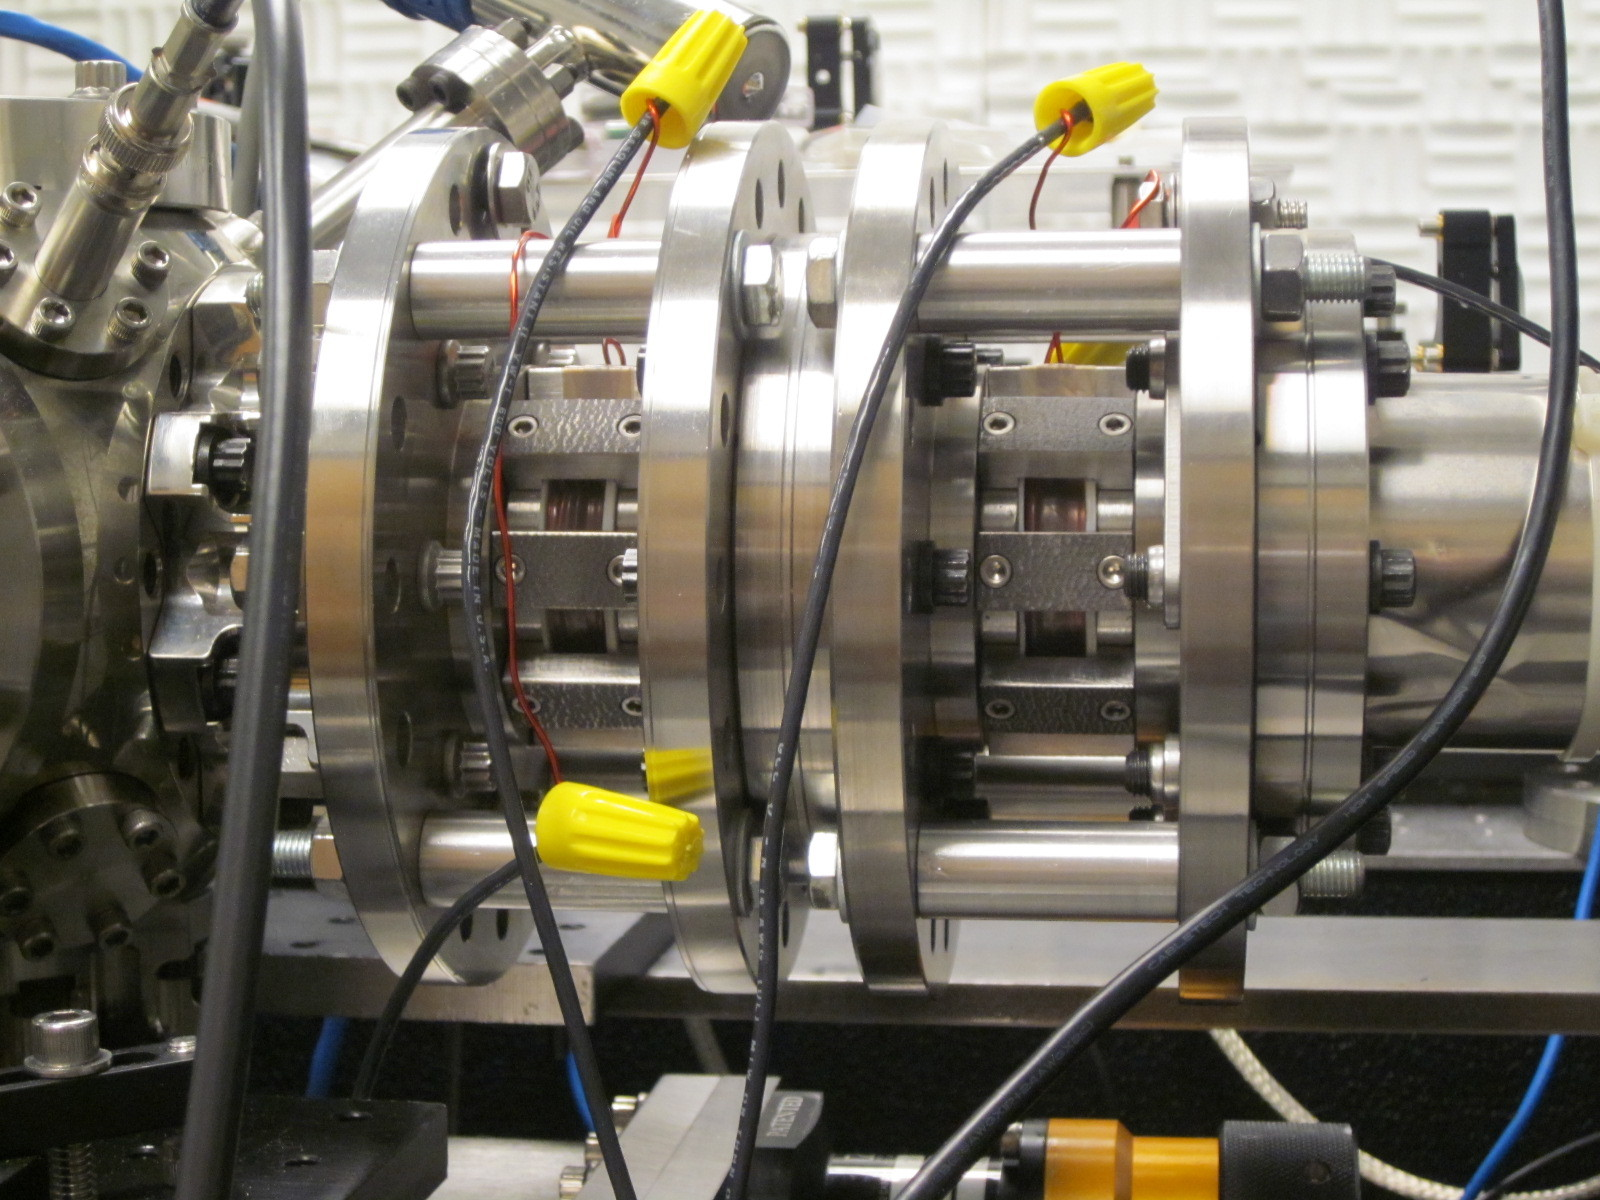
\includegraphics{maglens.jpg}
  \caption[Side-view picture of the employed two custom large-bore magnetic lenses]{
    Side-view of the two custom large-bore magnetic lenses designed and built at UIC, seen installed in the prototype UEM.
    The coils are visible as is high permeability shielding used for the pole-piece.
    The outer (larger) plates and struts are for structural integrity only.
  }
  \label{fig:maglens-pic}
\end{figure}

\subsection{Thermal Properties}

%TODO need reference for equation and \alpha_{Cu}
Since the lenses have no cooling devices, it was prudent to characterize the thermal response to a moderate current load.
Resistance of metals changes as a function of temperature by $ R = R_0 [ 1 + \alpha ( T - T_0 ) ] $, where $\alpha$ is a material contant; for copper, $\alpha = 3.9 * 10^{-3} \text{K}^{-1}$. 
One can calculate the temperature increase of the system by monitoring the change in resistance.
Maintaining a constant current of 4A through the lens, the voltage drop increased from 1.22V ($R_0 = 0.305\Omega$) to 1.25V ($R=0.3125\Omega$) as the lens warmed.
The resultant temperature increase is only $T - T_0 = 2\text{K}$.
This result is easily confirmed manually; the oxygen-free copper wire coils remain cool to the touch under these operating conditions.

